%!TEX root = ../Thesis.tex
%\chapter{Long chapter title with $\pi$ $π$ or π}
%\chapter{Long chapter title with \texorpdfstring{$\pi$ $π$ or π}{π π or π}}
\section{Deep Unsupervised 4D Seismic 3D Time-Shift Estimation with Convolutional Neural Networks}

%The abstract goes here.
\paragraph{Abstract:} We present a novel 3D warping technique for the estimation of 4D seismic time-shift. This unsupervised method provides a diffeomorphic 3D time shift field that includes uncertainties, therefore it does not need prior time-shift data to be trained. This results in a widely applicable method in time-lapse seismic data analysis. We explore the generalization of the method to unseen data both in the same geological setting and in a different field, where the generalization error stays constant and within an acceptable range across test cases. We further explore upsampling of the warp field from a smaller network to decrease computational cost and see some deterioration of the warp field quality as a result.

\subsection*{Key points:}
\begin{itemize}
    \item 3D time shift extraction
    \item Diffeomorphic constraint models geological intuition
    \item Unsupervised training does not need prior time shifts
    \item Generalizes to same field with different acquisition
    \item Generalizes to different field with differen geological setting
\end{itemize}

{\vfill\hfill\newline\fbox{\parbox{.97\textwidth}{\fullcite{dramsch20193dwarping}}}}

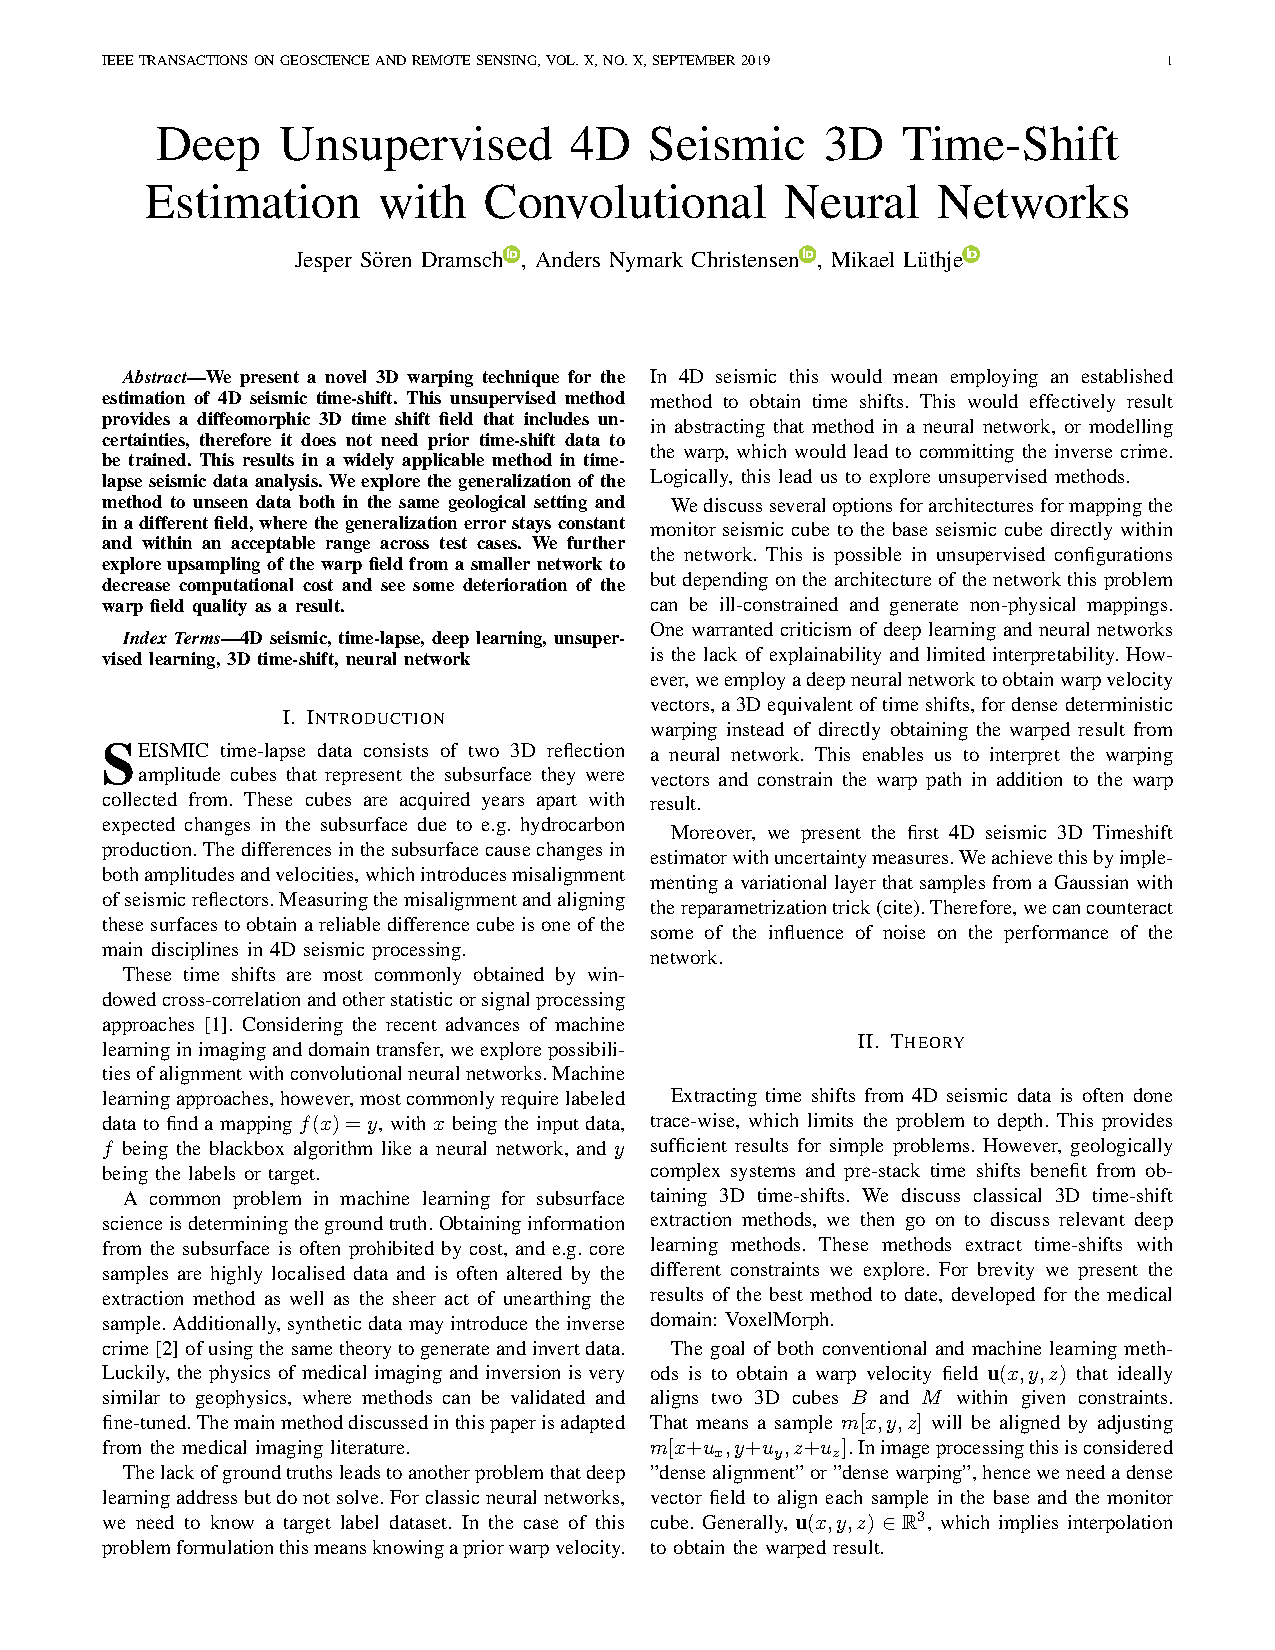
\includepdf[pages={1-13},width=1.2\textwidth,offset=0.7cm -1.5cm]{papers/2019.5}
